\chapter{Grundlagen}
\label{chap:grundlagen}

%\section{Analyse der Marsoberfläche}
%\label{sec:analysedermarsoberflache}

\section{Aufnahmen der Marsoberfläche}
\label{sec:mars_images}

Von der Marsoberfläche existieren verschiedenste Arten von Aufnahmen für unterschiedliche Analysen. Dabei kommt es auf gewisse Parameter, wie \zB die aufgenommene Wellenlänge, den Winkel zur Oberfläche, die Auflösung, Brennweite, Ort der Aufnahme und viele weitere an, ob ein Bild zur Analyse einer gewissen Eigenschaft geeignet ist.

Für die hier genutzten Anwendungsfälle eignen sich Instrumente am besten, die sichtbares Licht aufnehmen. Diese sollten in Graustufen, in diesem Einsatzbereich also panchromatisch, aufgenommen sein, da die Farbe der Oberfläche deren Analyse hier wenig beeinflusst. Der Vorteil von Graustufenaufnahmen besteht darin, dass nur ein drittel des Speichers bei den Berechnungen benötigt wird.

Des weiteren sollten die Bilder eine vergleichsweise hohe Auflösung haben, damit auch kleinere Merkmale gut erkannt werden können, es sollten aber auch weite Aufnahmen sein, damit mit einem Datensatz ein Großteil der Oberfläche analysiert werden kann.

Außerdem eignen sich Fotos gut, die senkrecht zur Oberfläche entstanden sind, so dass diese nicht verzerrt erscheint.

Unter Berücksichtigung dieser Faktoren ergeben sich \ua zwei geeignete Instrumente:
Die \textit{Context Camera (CTX)} des \textit{Mars Reconnaissance Orbiters} der NASA \cite{malin_07} und die \textit{High Resolution Stereo Camera (HRSC)} des \textit{Mars Express Orbiters} der ESA \cite{hrsc}. Für die eigentlichen Analysen werden Aufnahmen der CTX genutzt, da sie einen Großteil der Oberfläche abdecken, während die panchromatischen Bilder der HRSC zur Evaluierung genutzt wurden, da mit ihnen schon mehrere andere Algorithmen getestet wurden.

\section{Clustering}
\label{sec:clustering}


\section{Bildsegmentierung}
\label{sec:segmentierung}

Um in einem Eingabebild, wie \zB einer Aufnahme der Marsoberfläche, verschiedene Oberflächenstrukturen erkennen zu können, bedarf es eines Algorithmus zur Bildsegmentierung. Wie in \cite{bildsegmentierung_14} aufgeführt, beschreibt der Überbegriff der Bildsegmentierung oftmals den Ablauf des Pre-Processing eines Eingabebildes, gefolgt von der eigentlichen \textquote[\cite{bildsegmentierung_14}]{Segmentierung der Bilder in Regionen, Objekte mit geschlossenen Konturen oder Liniensegmente} und, je nach Anwendungsfall, der anschließenden Einordnung der einzelnen Segmente.

\section{Künstliche Intelligenz, maschinelles Lernen und Deep Learning}

\begin{wrapfigure}{r}{0.33\textwidth}
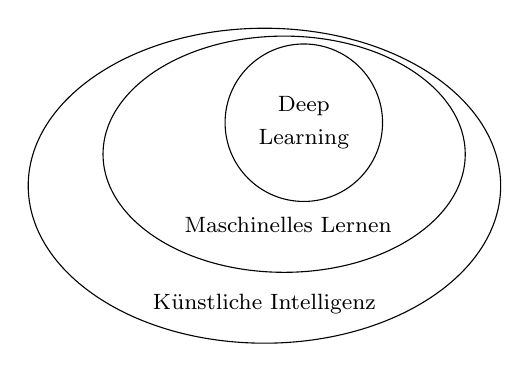
\begin{tikzpicture}
\draw (0,0) ellipse (3 and 2);
\draw (0,-1.5) node[align=center]{\footnotesize Künstliche Intelligenz};
\draw (0.25,0.4) ellipse (2.3 and 1.5);
\draw (0.3,-0.5) node[align=center]{\footnotesize Maschinelles Lernen};
\draw (0.5,0.8) ellipse (1 and 1);
\draw (0.5,0.8) node[align=center]{\footnotesize Deep\\\footnotesize Learning};
\end{tikzpicture}
\captionsetup{format=plain}
\caption{Relation zwischen künstlicher Intelligenz, maschinellem Lernen und Deep Learning, nach \cite[Kap.~1.1]{deeplearning_18}}
\label{fig:ai_ml_dl}
\end{wrapfigure}

Für den Begriff der künstlichen Intelligenz existieren viele Definitionen. Meistens wird mit ihm der Versuch bezeichnet, Maschinen, wie \zB Computern, eine Intelligenz beizubringen, die der des Menschen möglichst nahe sein sollte. Die Definition der Intelligenz ist selbst allerdings auch sehr unterschiedlich, laut einer Definition beschreibt Intelligenz \textquote{\textelp{} das Merkmal, das einem Wesen ermöglicht, angemessen und vorausschauend in seiner Umgebung zu funktionieren.}\footnote{\textquote[\cite{thequest_09}]{\textelp{} and intelligence is that quality that enables an entity to function appropriately and with foresight in its environment.}}

Während man in der klassischen Programmierung zur Lösung eines Problems sowohl Eingabedaten als auch Bearbeitungsregeln benötigt, so ändert sich dies beim maschinellen Lernen, einem Unterbegriff der künstlichen Intelligenz. Hier werden die Bearbeitungsregeln durch schon bekannte Ergebnisse -- passend zu den Eingabedaten -- ersetzt. Durch diese Kombination von Ein- und Ausgabewerten leitet die Maschine in der ersten Phase, auch Training genannt, so selbst die Bearbeitungsregeln ab, und kann sie in der zweiten Phase auf neue, unbekannte Eingabewerte anwenden. Diese Bearbeitungsregeln bestehen aus generierten Formeln und beruhen auf rein statistischen Annahmen darüber, mit welcher Wahrscheinlichkeit eine gewisse Eingabe zu einer anderen gewissen Ausgabe führt. \cite{deeplearning_18} 

Deep Learning -- meist synonym mit neuronalen Netzen genutzt -- wird oftmals als eine Weiterentwicklung oder Optimierung des maschinellen Lernens betrachtet: Statt einer Menge von Formeln, die das Resultat bestimmen sollen, setzt man hier auf mehrere Schichten, auch Layers genannt, von vergleichsweise einfachen linearen Funktionen, um zum gewünschten Ergebnis zu kommen. In diesem Kontext wird ein Knoten, also eine Funktion auch als Neuron bezeichnet. Die Aneinanderkettung dieser verschiedenen Schichten führt dazu, dass zwischen ihnen eine immer abstrahiertere Form der Eingabedaten entsteht, damit sind sie in ihrer Funktionsweise an die des menschlichen Gehirns angelehnt, welches sich auch aus einer Großzahl von hintereinandergeschalteten Neuronen zusammensetzt. Jedes Neuron ist mit mehreren Neuronen aus der Schicht vor und nach ihm vernetzt. \cite{schmidhuber_15} Während das Netzwerk trainiert wird, passen die einzelnen Knoten jeweils zwei Werte an: Wie sehr sie die Ausgabe der jeweils vorherigen Schicht aus Knoten gewichten, und die Mindestgrenze anhand welcher sie bestimmen, ob sie überhaupt einen Wert an die nächste Schicht ausgeben. Diese Gewichtungen sind anfangs zufällig bestimmt. \cite{hardesty_17, schmidhuber_15}

Obwohl einfache Versionen neuronaler Netze schon seit vielen Jahrzehnten in der Informatik genutzt werden, wurden mit ihnen in den letzten Jahren neue Durchbrüche in verschiedensten Bereichen erzielt. Dieser Umschwung ist darauf zurückzuführen, dass mit dem Fortschritt der Technik nun auch große Netzwerke effizient ausgeführt werden können.




\section{Convolutional Neural Networks}
\label{sec:cnn}

Ein Convolutional Neural Network beschreibt ein Neuronales Netzwerk, welches eine Convolutional Layer enthält. Eine Convolutional Layer enthält ihre Eingaben von mehreren Datenpunkten der vorherigen Schicht: Das (meist rechteckige) Fenster der Eingabedaten dieser Schicht gleitet somit schrittweise über die Ausgabe der vorherigen Schicht. \cite{schmidhuber_15} Dies hat den Vorteil, dass die Größe der darauf folgenden Schicht verringert wird (was zu einer besseren Performance führt). Ein weiterer Pluspunkt besteht darin, dass insbesondere bei der Bildanalyse gleiche Objekte an verschiedenen Positionen und in verschiedenen Größen besser erkannt werden können. \cite{szegedy_15}

Aus diesen Gründen erfreuen sich Convolutional Neural Networks insbesondere in der Bildanalyse (wie \zB bei der Objekterkennung) großer Beliebtheit.

\section{Convolutional Layer}
\label{sec:conv}

\section{Pooling Layer}
\label{sec:pooling}

\section{Backpropagation}
\label{sec:backpropagation}¸